\chapter{Swing-Up Design}\label{sec:swing-upDesign}
In this chapter a swing-up controller is designed based on \cite{kjAastrom}. The pendulum is started at rest, $\theta = \pi$, angle convention is specified in \autoref{fig:mechanicalDrawing}. The idea of the swing-up controller is to increase the mechanical energy in the system until it matches that of the desired end state, which is the upright position at rest, that is, $\theta = 0$ and $\dot{\theta} = 0$. The minimum energy in the system is the starting position at rest, which is considered to be zero as mentioned in the \textit{Model} \autoref{sec:model}. So the target energy is $E_{\mathrm{eq}} = 2 m g l$, that is, the potential energy of the pendulum in the unstable equilibrium.

Consider the pendulum dynamics from \autoref{eq:energyDerivedDynamicEquation1},
\begin{flalign}
&& J \ddot{\theta} - m l \cos \theta \ddot{x}_c - m g l \sin \theta  &= 0 \ \ \ , &  \unit{N \cdot m}   \label{eq:pendulumDynamics}
\end{flalign}
where $J = m l^2$ is the inertia and the pendulum friction is assumed to be zero. This equation captures the behavior of the pendulum corresponding to some acceleration $\ddot{x}_c$ at the pivot point. This acceleration is viewed as the control input for now. The force needed to achieve this acceleration is considered in the end of the design. It is further convenient to describe the energy of the pendulum with the coordinate frame fixed at its pivot point, see \autoref{fig:fixedCooredinateSystem}.
%
\begin{figure}[H]
  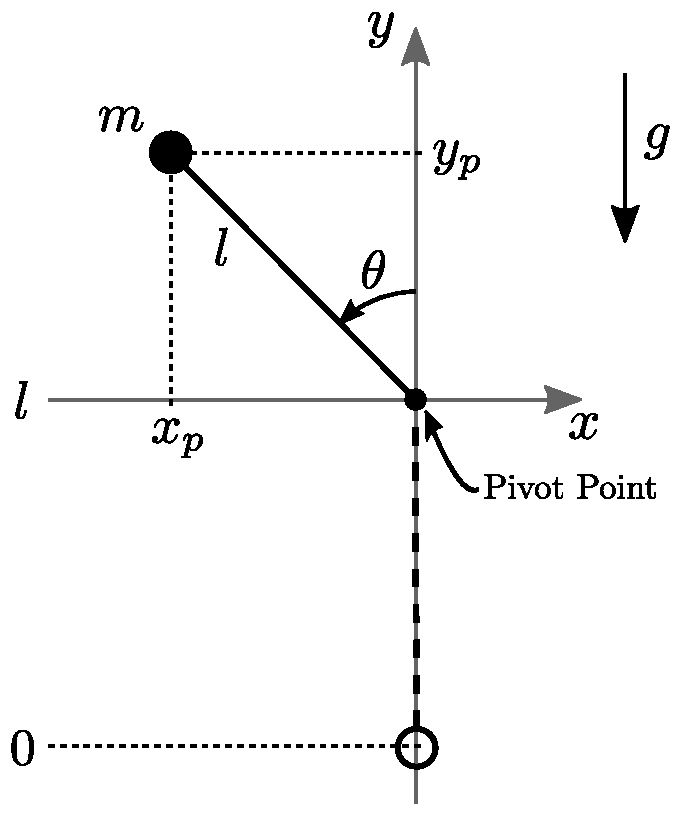
\includegraphics[width=.3\textwidth]{figures/fixedCooredinateSystem}
  \caption{The energy used in the swing-up controller is described using this convention, where the coordinate frame is fixed at the pivot point of the pendulum. The zero reference is placed as before s.t. all energies are positive.}
  \label{fig:fixedCooredinateSystem}
\end{figure}
%
From \autoref{fig:fixedCooredinateSystem}, the conversion from excessive to generalized coordinates is given by,
\begin{flalign}
&& x_p  &= -l \sin \theta   \ \ \ ,\ \ \ y_p = l(\cos \theta + 1)  \ \ \ ,\ \ \ \dot{x}_p = -l \cos \theta \dot{\theta}  \ \ \ ,\ \ \ \dot{y}_p = -l \sin \theta \dot{\theta}  \ \ \ . &&     \label{eq:cooredinateConvertFixed}
\end{flalign}
The mechanical energy in this coordinate frame is then,
\begin{flalign}
&& E_p &= m g y_p + \tfrac{1}{2} m \dot{x}_p^2 + \tfrac{1}{2} m \dot{y}_p^2  &  \unit{J}   \label{eq:pendulumEnergy1} \\
&& E_p &= m g l (\cos \theta +1) + \tfrac{1}{2} m (-l \cos \theta \dot{\theta})^2 + \tfrac{1}{2} m (-l \sin \theta \dot{\theta})^2  &  \unit{J}   \label{eq:pendulumEnergy2} \\
&& E_p &= m g l (\cos \theta +1) + \tfrac{1}{2} J (\cos^2 \theta  + \sin^2 \theta )\dot{\theta}^2  &  \unit{J}   \label{eq:pendulumEnergy3} \\
&& E_p &= \tfrac{1}{2} J \dot{\theta}^2 + m g l (\cos \theta +1) \ \ \ . &  \unit{J}   \label{eq:pendulumEnergy4}
\end{flalign}
%
A Lyapunov function candidate is proposed,
\begin{flalign}
&& V &= \tfrac{1}{2} E_\Delta ^2 \ \ \ ,  \hspace{5cm}  &&&  \label{eq:lyapunovCandidate} 
\end{flalign}
where $E_\Delta$ is the difference in energy in relation to the unstable equilibrium,
%
\begin{flalign}
&& E_\Delta &= E_p  - E_{\mathrm{eq}} &  \unit{J}   \label{eq:energyDelta1} \\
&& E_\Delta &= \tfrac{1}{2} J \dot{\theta}^2 + m g l (\cos \theta +1) - 2 m g l &  \unit{J}   \label{eq:energyDelta2} \\
&& E_\Delta &= \tfrac{1}{2} J \dot{\theta}^2 + m g l (\cos \theta -1)   \ \ \ .  & \unit{J} \label{eq:energyDelta3}
\end{flalign}
%
The derivative of $E_\Delta$ from \autoref{eq:energyDelta3} along the system \autoref{eq:pendulumDynamics} is found to,
\begin{flalign}
&& \dot{E}_\Delta &= J \dot{\theta} \ddot{\theta} - m g l \sin \theta \dot{\theta}  &&&   \label{eq:energyDeltaDerivative1} \\
&& \dot{E}_\Delta &= \dot{\theta} ( m l \cos \theta \ddot{x}_c + m g l \sin \theta )  - m g l \sin \theta \dot{\theta}    &&&   \label{eq:energyDeltaDerivative2} \\
&& \dot{E}_\Delta &=  m l \cos \theta \dot{\theta} \ddot{x}_c \ \ \ .   &&&   \label{eq:energyDeltaDerivative3}
\end{flalign}
The Lyapunov function candidate, \autoref{eq:lyapunovCandidate}, is continuously differentiable in the entire $\mathbb{R} ^2$ \fxnote{brush up on stability criteries}. Its derivative is evaluated to find a stabilizing controller,
%
\begin{flalign}
&& \dot{V} &= E_\Delta \dot{E}_\Delta   \hspace{3cm}  &&&  \label{eq:lyapunovDerivative1}  \\
&& \dot{V} &= E_\Delta m l \cos \theta \dot{\theta} \ddot{x}_c  \leq 0  \ \ \ .  \hspace{3cm}  &&&  \label{eq:lyapunovDerivative2} 
\end{flalign}
%
The acceleration, $\ddot{x}_c$, is then designed to satisfy the stability criterion in \autoref{eq:lyapunovDerivative2},
\begin{flalign}
&& \dot{V} &= m l E_\Delta \cos \theta \dot{\theta} (-E_\Delta \cos \theta \dot{\theta})     \hspace{2cm}  &&&  \label{eq:lyapunovDerivativeControlled1} \\
&& \dot{V} &= -m l (E_\Delta \cos \theta \dot{\theta})^2  \leq 0  \ \ \ ,  \hspace{2cm}  &&&  \label{eq:lyapunovDerivativeControlled2} 
\end{flalign}
further a tuning parameter, $k>0$, is introduced such that the control law for acceleration of the pivot point is,
\begin{flalign}
&& \ddot{x}_c &= -k E_\Delta \cos \theta \dot{\theta}  \ \ \ .  \hspace{4cm}  &&&  \label{eq:accControlLaw} 
\end{flalign}



